% Define document class
\documentclass[preprint]{aastex63}
\usepackage{tabularx}
\usepackage{amsmath}

\begin{document}

% Title
\title{Earth's Impact History and the Timing of the Origin of Life}

% Authors
\author{Nicholas F. Wogan}
\affiliation{Department of Earth and Space Sciences, University of Washington, Seattle, WA 98195}
\affiliation{Virtual Planetary Laboratory, University of Washington, Seattle, WA98195}

\author{David C. Catling}
\affiliation{Department of Earth and Space Sciences, University of Washington, Seattle, WA 98195}
\affiliation{Virtual Planetary Laboratory, University of Washington, Seattle, WA98195}

\author{Kevin J. Zahnle}
\affiliation{Space Science Division, NASA Ames Research Center, Moffett Field, CA 94035}
\affiliation{Virtual Planetary Laboratory, University of Washington, Seattle, WA98195}

\begin{abstract}
Big impacts on the early Earth would have created highly reducing atmospheres that generated molecules needed for the origin of life, such as nitriles. However, such impactors can be followed by impactors that were still sufficiently big to vaporize the ocean and destroy any incipient life. In this scenario, a post-impact reducing atmosphere needs to be followed by a lack of subsequent sterilizing impacts for life to persist. Using what we know about the impact history of early Earth and what is needed to generate post-impact highly reducing atmospheres, we show that  the median timing of biopoesis in this impact-driven scenario was $\sim 4.35$ Ga. However, uncertainties are large because impact bombardment is inherently stochastic, so biopoesis could have occurred in $\sim 0.5$ billion year window from 4.45 to 3.9 Ga within 95\% uncertainties of our model. Claims of a far narrower window for the origin of life are unsupported. In our optimistic scenario for life starting from post-impact reducing atmospheres, we find that biopoesis is possible in 92\% of stochastic impact realizations. This potentially bodes well for life on rocky planets elsewhere because these will have experienced an early episode of enhanced impact bombardment given how planets form.
\end{abstract}

\section{Introduction}

\citet{Benner_2020} argued that the most likely time for the origin of life in an RNA-world scenario would have been $4.36 \pm 0.1$ Ga in the wake of a $2 \times 10^{22}$ kg ($\sim 2100$ km) asteroid impact which they called Moneta. They suggested that iron delivered by Moneta's core would have reacted with impact-vaporized ocean water to generate a reducing Hadean atmosphere conducive to the photochemical generation of essential prebiotic molecules like HCN. This transient period could have been a window of opportunity for the origin of RNA and, ultimately, life.

A single Moneta impact could also explain the highly-siderophile elements (i.e. iron-loving, abbreviated HSEs) in the Moon's and the Earth's mantles. During the moon-forming impact, most all HSEs should have been sequestered in each planetary core, so extant mantle HSEs are commonly interpreted as evidence for late-accretion impactors. Earth's mantle has substantially more HSEs than the Moon by an amount that cannot be accounted for by Earth's greater gravitation cross section \citep{Day_2015}. A single massive Moneta impact could explain the Earth-Moon HSE discrepancy because, by the statistics of small numbers, Moneta could have missed the moon and hit the Earth \citep{Bottke_2010}.

However, the lunar HSE depletion has explanations that do not require a Moneta impact. Lunar HSEs could have been lost to space during impact-delivery because of the Moon's small gravity \citep{Kraus_2015}. Alternatively, HSEs delivered to the Moon during its $\sim 150$ million-year magma ocean could have been sequestered in the core due to iron sulfide exsolution \citep{Morbidelli_2018,Rubie_2016}. Finally, there is some chance that the Earth's HSEs do not record late impacts because the Moon-forming impact delivered HSEs \citep{Sleep_2016}, or because HSEs are gradual core contributions over time from mantle plumes \citep{Halliday_2023,Mundl_2020}. If indeed Earth's HSEs reflect asteroid bombardment after the Moon formed, then the HSEs can be explained by multiple $\sim 500$ to 2000 km impacts rather than a single big ($\sim 2100$ km) collision.

Recently, \citep{Wogan_2023} use photochemical models of post-impact atmospheres to show that impacts significantly smaller than Moneta can efficiently produce prebiotic molecules. In their simulations, impactor iron equilibrates with vaporized ocean water to generate atmospheric H$_2$, and CH$_4$ and NH$_3$ form thermochemically as the reducing steam atmosphere cools. Once steam condense to an ocean, subsequent photochemistry of the Titan-like atmosphere produces prebiotic nitriles. Modeling shows that the production of both HCN and HCCCN only occurs when $\mathrm{CH_4} / \mathrm{CO_2} \gtrsim 0.1$ while the atmosphere is hazy. In an optimistic scenario, which includes nickel catalyzed methane production, modeling suggests that $\mathrm{CH_4} / \mathrm{CO_2} > 0.1$ (i.e. significant nitriles) occurs for impacts $> 4 \times 10^{20}$ kg. In a pessimistic modeling case, which assumes only a fraction of impactor iron reacts with the atmosphere \citep{Citron_2022}, a $> 5 \times 10^{21}$ kg impactor is required to produce substantial HCN and HCCCN. Regardless of uncertainty, \citet{Wogan_2023} show that an impactor much smaller than Moneta could spark an origin of life, and that the \citet{Benner_2020} estimated timing for biopoesis could be inaccurate because it is based on Moneta.

Here, we use the \citet{Wogan_2023} results, along with Monte-Carlo simulations of Earth's impact history to make an alternative estimate for when life most likely emerged during an RNA-first process. Our calculations accounts for the possibility of planet sterilization by impacts that vaporize the ocean \citep{Sleep_1989}. We assume that an ``origin of life impact'' is one that produces significant prebiotic molecules and is not subsequently followed by an ocean-vaporizing impact that destroys the biosphere without rekindling it. By considering the fraction of stochastic impact realizations that do not have an ``origin of life impact'', we also estimate the probability of life beginning on the early Earth if we were to rerun the tape.

\section{Methods}
The rate impacts hit Earth bigger than mass $m$ at age $t$ is given by

\begin{equation}
  f(t,m) = F_0(t) S_0(m)
\end{equation}
Here, $S_0(m)$ is the size-frequency distribution of impactors normalized to a reference mass $m_0$ so that $S_0(m_0) = 1$. Also, $F_0(t)$ is the number of impacts per billion years with mass greater than $m_0$.

We assume the size-frequency distribution of impactors is identical to the main-belt asteroids \citep[Extended Data Figure 1,][]{Marchi_2014}. Data for the frequency of main-belt asteroids only extends down to about 1 km diameter ($= 1.3 \times 10^{12} $ kg). To extend the distribution to smaller objects, we use the observed 1400 ratio between the frequency of $> 1$ km and $> 20$ km craters on the Moon. \citet{Morbidelli_2018} uses crater scaling relations to show that 1 km and 20 km craters on the Moon corresponds to 50 m and 1 km asteroids, respectively. The largest main belt asteroid is $\sim 1000$ km, so we log-linearly extrapolate to larger impactors (Figure \ref{fig:sfd_and_flux}). Finally, we normalize the size-frequency distribution to the impact mass required to make a 1 km crater on the moon (50 m object, $m_0 = 1.64 \times 10^{8}$ kg). Figure \ref{fig:sfd_and_flux}a shows the resulting size-frequency distribution.

\begin{figure}
  \centering
  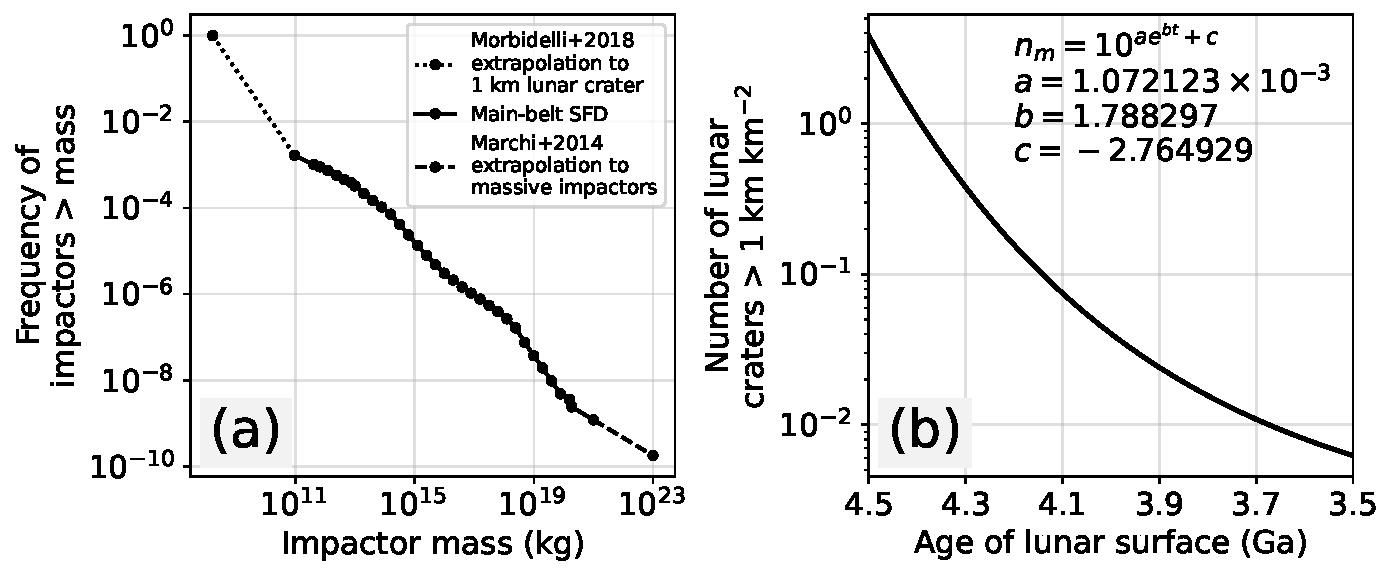
\includegraphics[width=1.0\textwidth]{figures/SFD_and_flux.pdf}
  \caption{Caption}
  \label{fig:sfd_and_flux}
\end{figure}

The flux of impactors, $F_0(t)$, can be estimated from the lunar cratering record. We adopt the accretionary tail scenario discussed in \citet{Morbidelli_2018}. In other words, we assume that the ``late heavy bombardment'' did not happen \citep{Cartwright_2022,Hartmann_2019,Zellner_2017}, and that the impact flux on Earth was constantly decreasing throughout the Hadean eon. Figure \ref{fig:sfd_and_flux}b shows $n_m$, our assumed lunar impact history taken from \citet{Morbidelli_2018} (red line in their Figure 5).

Extrapolating the lunar impact history to Earth requires correcting for Earth's greater gravitational attraction. Assuming the approach velocity of impactors far from the Earth and Moon was on average 18 km/s \citep{Morbidelli_2018}, then Earth should receive $s_0 = 1.36$ times more impacts per surface area than the Moon. Therefore, the number of impacts on Earth is

\begin{equation}
  N_0 = A_\oplus s_0 n_m = A_E s_0 10^{a e^{b t} + c}
  \label{eq:num_earth_impacts}
\end{equation}
Equation \eqref{eq:num_earth_impacts} also accounts for Earth's surface area ($A_\oplus$), making $N_0$ the number of impacts on Earth since age $t$ that cause a crater $> 1$ km on the moon. As discussed previously, \citet{Morbidelli_2018} use crater scaling relations to show that a 1 km lunar crater corresponds to a 50 m object with mass $m_0 = 1.64 \times 10^8$ kg.

The derivative of $N_0$ gives the flux, $F_0$:

\begin{equation}
  F_0(t) = \frac{d N_0}{dt}
\end{equation}
The average number of impacts on Earth between time $t_1$ and $t_2$ with mass greater than $m$ is then

\begin{align}
\begin{split}
  N(m,t_1,t_2) &= \int_{t_1}^{t^2} f(t,m) dt \\
  &= S_0(m) \int_{t_1}^{t^2} \frac{d N_0}{dt} dt \\
  &= S_0(m) A_\oplus s_0 \left( 10^{a e^{b t_2} + c} - 10^{a e^{b t_1} + c} \right)
\end{split}
\end{align}

To simulate impact histories, we consider a fine grid of impactor masses between $10^{12}$ and $10^{23}$ kg, and a grid of times between 4.5 and 3.5 Ga. Indexes $j$ and $i$ indicate the mass and time grid cells respectively, while, for example, $j-\frac{1}{2}$ and $j+\frac{1}{2}$ indicate the edges of the grid cell. We can compute the expected number of impacts within a mass and time grid cell with the following

\begin{equation}
  \overline{N}_{ij} = N(m_{j-\frac{1}{2}},t_{i-\frac{1}{2}},t_{i+\frac{1}{2}}) - N(m_{j+\frac{1}{2}},t_{i-\frac{1}{2}},t_{i+\frac{1}{2}})
\end{equation}
Next, we sample a Poisson distribution for each $\overline{N}_{ij}$, giving a stochastic number of impacts in each mass and time grid cell which constitutes an impact history. Performing this sampling thousands of times captures many of the possible impact histories. We only keep impact histories that accrete a total mass of $2 \times 10^{22}$ and $6 \times 10^{22}$ kg because this is approximately the mass implied by the HSEs in Earth's mantle. This range of masses is based on \citet{Day_2015} who used mantle HSEs to suggest that the Earth was impacted by $\sim 3 \times 10^{22}$ to $4.8 \times 10^{22}$ kg of material, but we choose a wider range of masses because HSEs could have been lost to Earth's core or to space during impacts \citep{Marchi_2018}.

Our final step is to assign impact velocities to each collision in the many sampled impact histories. Appendix Figure \ref{fig:velocity_distribution} shows Earth's impact velocity distribution. We created this distribution using the JPL database of close approaches to Earth by small bodies \citep{Park_2023}, considering all close approach asteroids within 0.05 AU to Earth. The database gives the approach velocity of each asteroid far from Earth, so we compute the impact velocity by accounting for Earth's gravitational energy.

The final collection of sampled impact histories can then be used to compute impact statistics which are relevant to the timing and likelihood of the origin of life.

\section{Results}

\begin{figure}
  \centering
  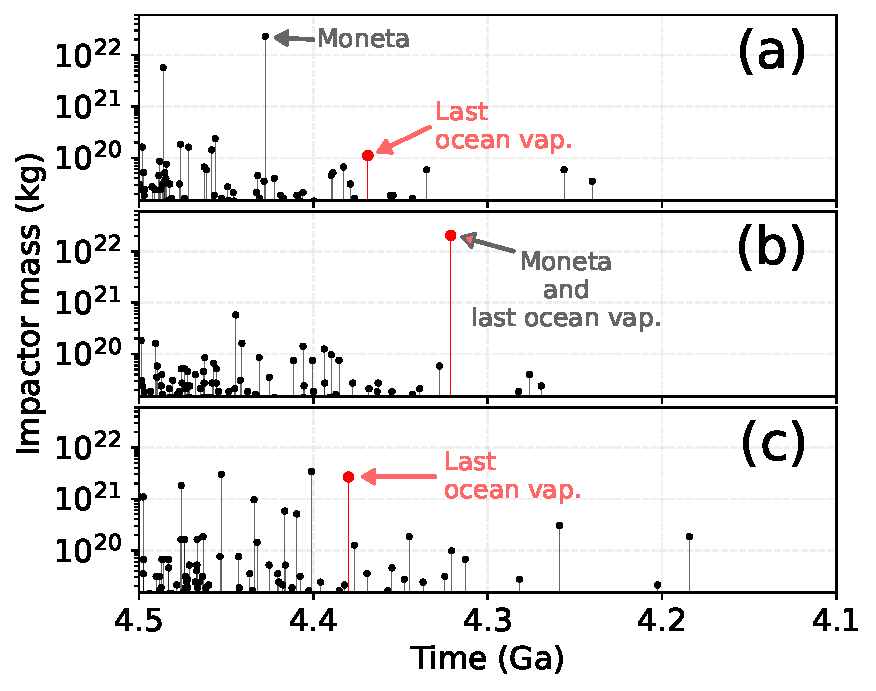
\includegraphics[width=0.65\textwidth]{figures/example_impact_histories.pdf}
  \caption{Caption}
  \label{fig:example_impact_histories}
\end{figure}



\section{Discussion and Conclusions}

\section*{Acknowledgements}

N.F.W. and D.C.C. were supported by the Simon's Collaboration on Origin of Life Grant 511570 (to D.C.C.). Also, N.F.W., D.C.C., and K.J.Z. were supported by NASA Astrobiology Program Grant 80NSSC18K0829 and benefited from participation in the NASA Nexus for Exoplanet Systems Science research coordination network. N.F.W. and D.C.C. also acknowledge support from Sloan Foundation Grant G-2021-14194. K.J.Z. was supported by NASA Exobiology Grant 80NSSC18K1082.

\appendix

\renewcommand{\thefigure}{A\arabic{figure}}
\renewcommand{\thetable}{A\arabic{table}}
\setcounter{figure}{0}
\setcounter{table}{0}

\begin{figure}
  \centering
  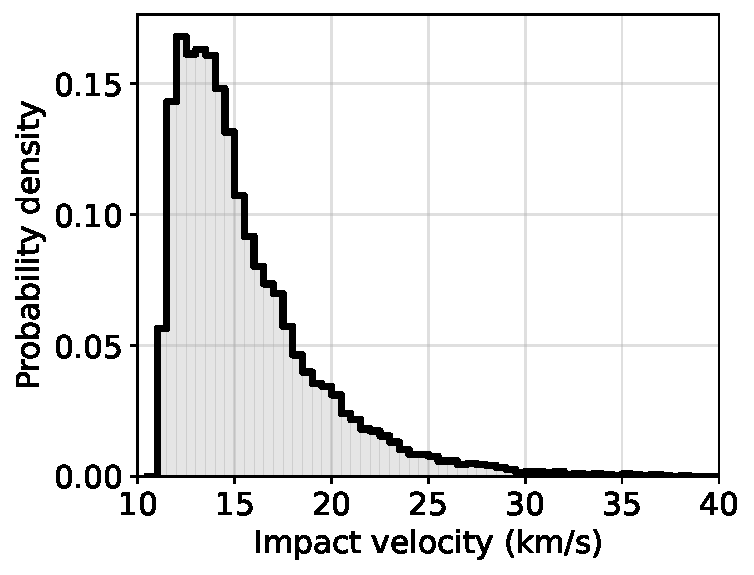
\includegraphics[width=0.4\textwidth]{figures/velocity_distribution.pdf}
  \caption{Caption}
  \label{fig:velocity_distribution}
\end{figure}


\bibliography{bib}
\bibliographystyle{aasjournal}

\end{document}
